%
% File emnlp2019.tex
%
%% Based on the style files for ACL 2019, which were
%% Based on the style files for EMNLP 2018, which were
%% Based on the style files for ACL 2018, which were
%% Based on the style files for ACL-2015, with some improvements
%%  taken from the NAACL-2016 style
%% Based on the style files for ACL-2014, which were, in turn,
%% based on ACL-2013, ACL-2012, ACL-2011, ACL-2010, ACL-IJCNLP-2009,
%% EACL-2009, IJCNLP-2008...
%% Based on the style files for EACL 2006 by 
%%e.agirre@ehu.es or Sergi.Balari@uab.es
%% and that of ACL 08 by Joakim Nivre and Noah Smith

\documentclass[11pt,a4paper]{article}
\usepackage[hyperref]{emnlp-ijcnlp-2019}
\usepackage{times}
\usepackage{latexsym}
\usepackage{graphicx}  %%% for including graphics
\usepackage{booktabs}


\usepackage{url}

%\aclfinalcopy % Uncomment this line for the final submission

%\setlength\titlebox{5cm}
% You can expand the titlebox if you need extra space
% to show all the authors. Please do not make the titlebox
% smaller than 5cm (the original size); we will check this
% in the camera-ready version and ask you to change it back.

\newcommand\BibTeX{B{\sc ib}\TeX}
\newcommand\confname{EMNLP-IJCNLP 2019}
\newcommand\conforg{SIGDAT}

\title{Instructions for \confname{} Proceedings}

\author{First Author \\
  Affiliation / Address line 1 \\
  Affiliation / Address line 2 \\
  Affiliation / Address line 3 \\
  {\tt email@domain} \\\And
  Second Author \\
  Affiliation / Address line 1 \\
  Affiliation / Address line 2 \\
  Affiliation / Address line 3 \\
  {\tt email@domain} \\}

\date{}

\begin{document}
\maketitle
\begin{abstract}
\end{abstract}


\newcommand{\refexp}[1]{\textsl{#1}}
\newcommand{\word}[1]{\textsl{#1}}
\newcommand{\cat}[1]{\textsc{#1}}
\newcommand{\vgenome}{VisualGenome\xspace}
\newcommand{\ra}{$\rightarrow$}

\newcommand{\sz}[1]{\textcolor{blue}{\emph{//sz: #1//}}}


\section{Introduction}

The real-world objects that we interact with in our every-day life can be categorized into many thousands and maybe millions of categories. And even a single object can be member of many categories, i.e.\ at different taxonomical levels or in different parts of a taxonomy. For instance, both objects in Figure \ref{fig:cake} are at once instances of \cat{cake}, \cat{cheesecake}, \cat{dessert}, \cat{sweet}, \cat{pastry}, \cat{food} etc. Hence, when speakers name objects, e.g.\ when referring, they have to select a lexical item from a complex network of concepts and competing lexical alternatives.


\begin{figure}[htbp]
\begin{center}
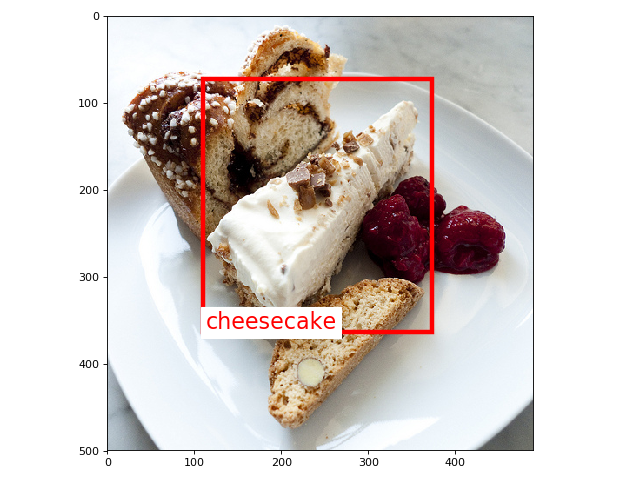
\includegraphics[height=3cm]{Figures/cheescake.png}
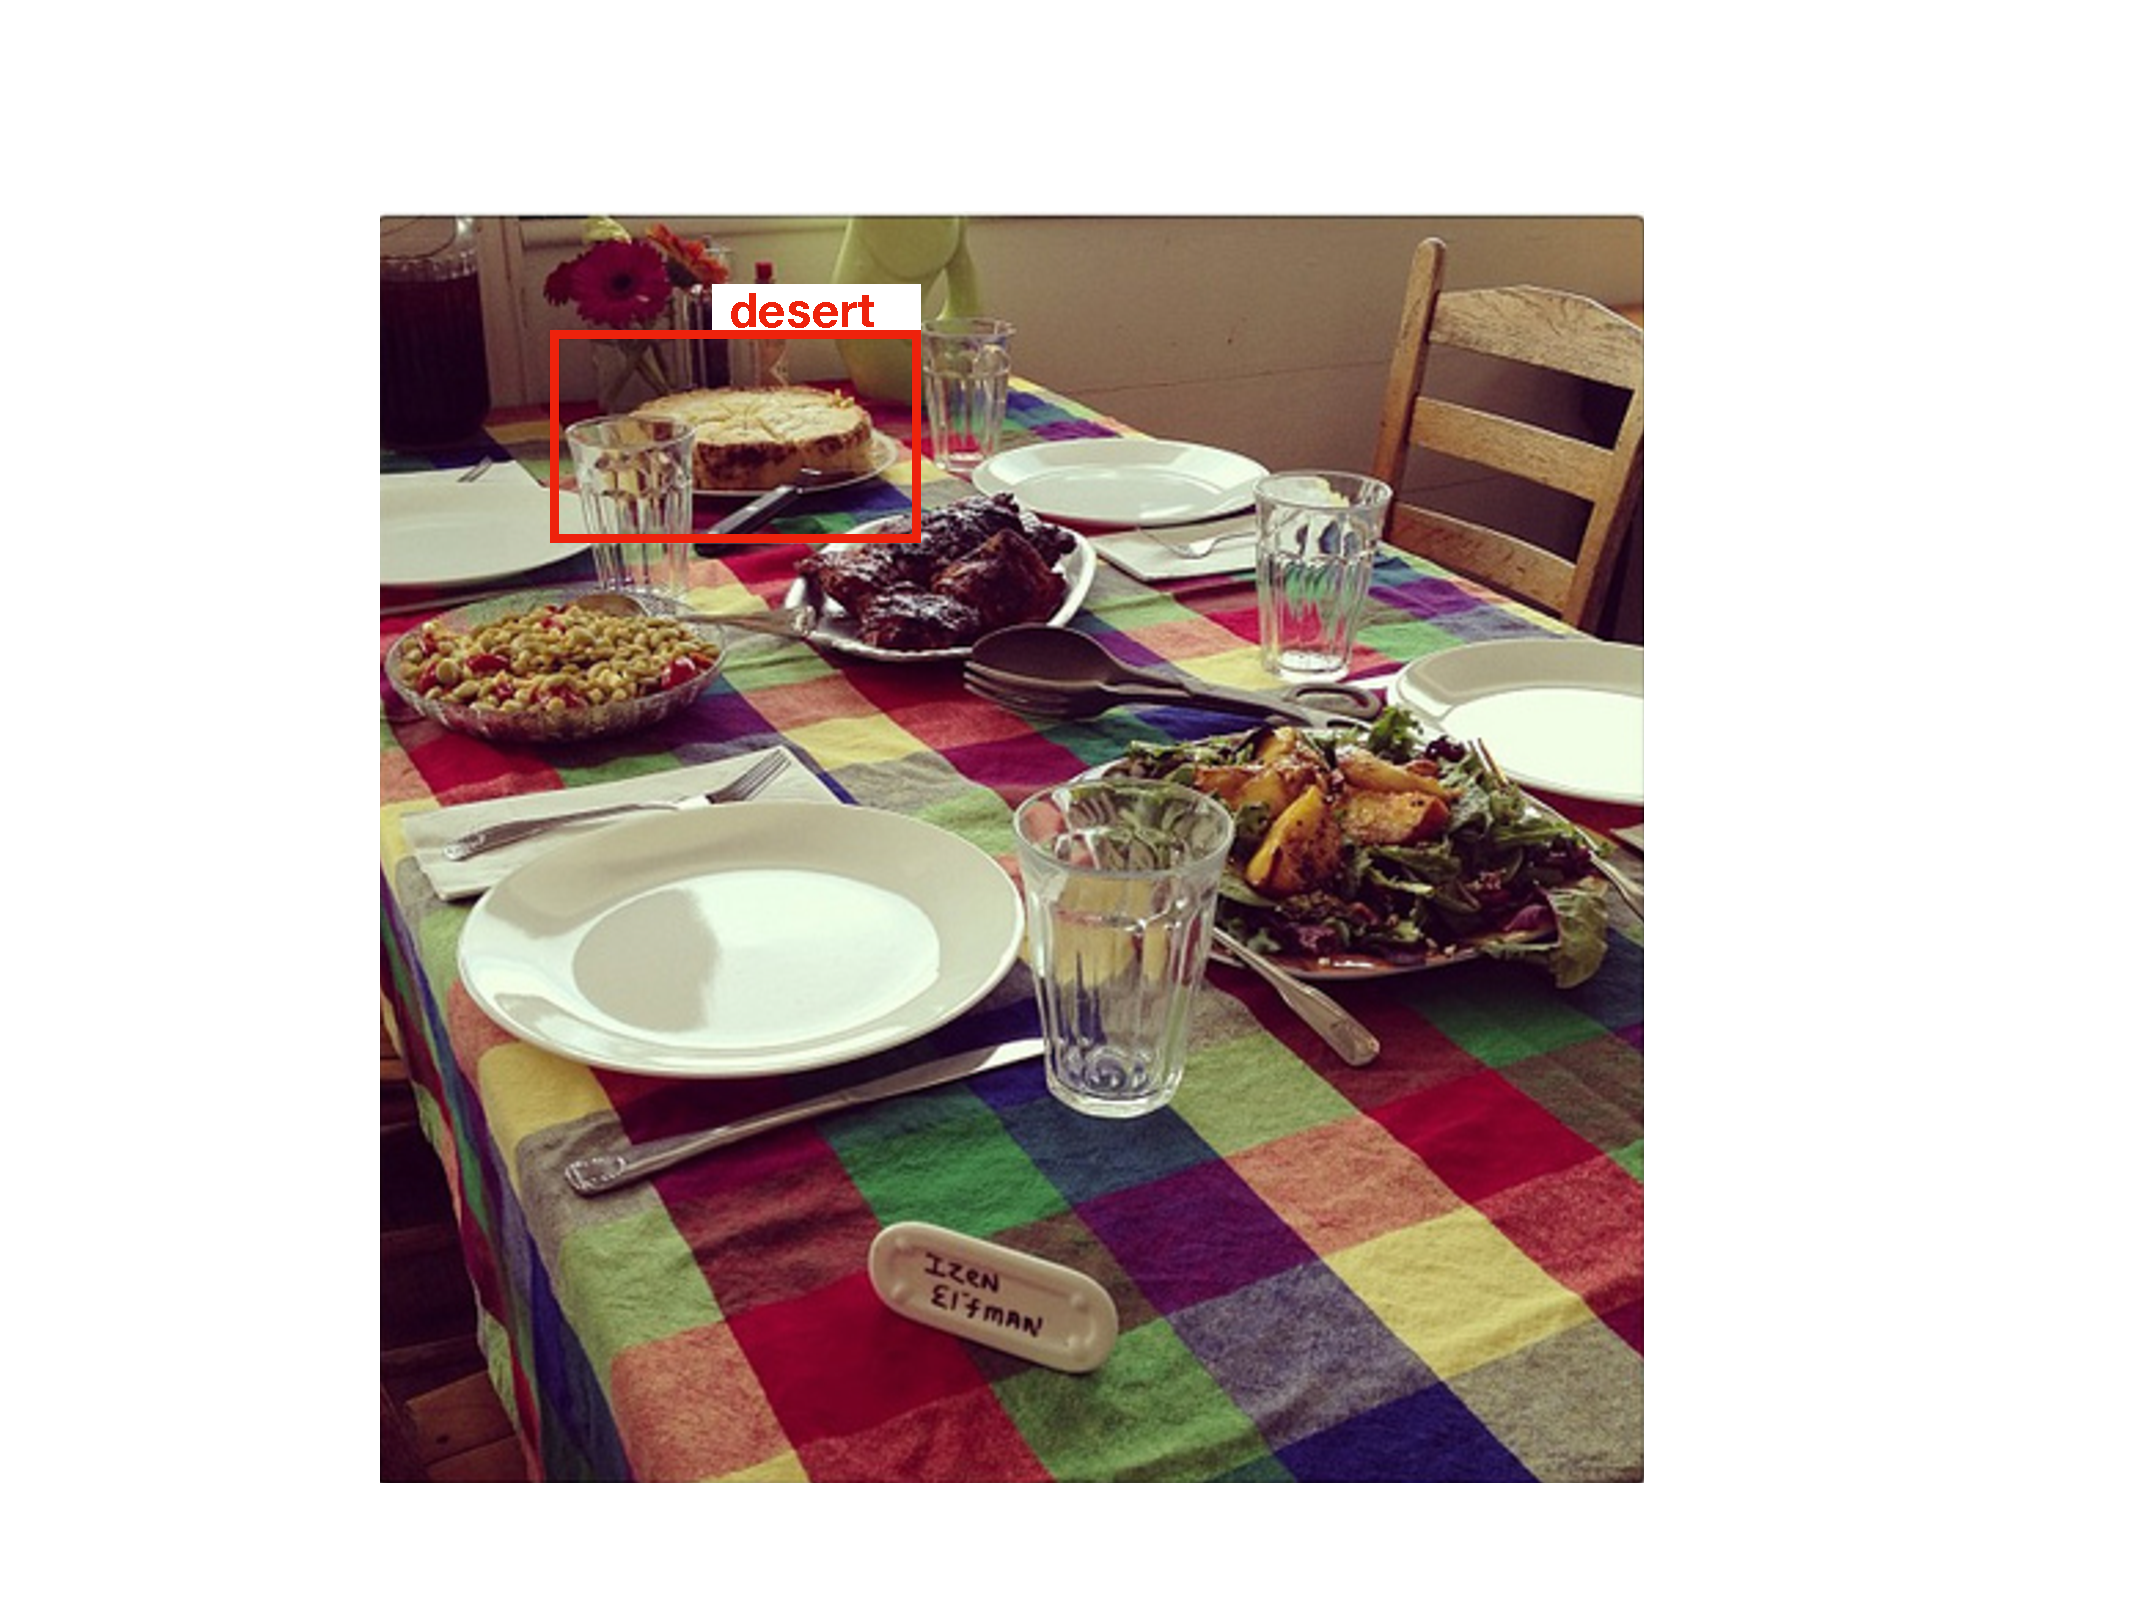
\includegraphics[height=3cm]{Figures/cheesecak2.pdf}
\caption{Two objects of the same type of cake, with different names in VisualGenome}
\label{fig:cake}
\end{center}
\end{figure}

To date, research in NLP has surprisingly little to say about object naming, despite the fact that
 there has been a recent explosion of interest in various, and even complex, language \& vision tasks ranging from image captioning \cite{fangetal:2015,devlin:imcaqui,Bernardietal:automatic} to e.g.\ visual dialogue \cite{das2017visual,vries2017guesswhat}. 
In contrast, closely related areas, such as computer vision and cognitive science, have investigated very related tasks in quite some depth: object recognition systems developed in the area of computer vision  are now able to classify images into thousands of different categories (e.g.\  \newcite{googlenet}).
Furthermore, work on concepts, following the seminal work by Rosch, suggests that objects are typically conceptualized at a preferred level of specificity called the \textbf{entry-level}. Psycho-linguistic studies have been able to support this theory based on collections of so-called object naming norms. 

This paper aims at addressing the genuinely linguistic questions revolving around the phenomenon of object naming by (i) presenting a collection of high-quality, large-scale naming data,  and (ii) analysis methods for this data and (iii) a first baseline model that accounts for the semantic flexibility of names for objects in real-world images. From computer vision, we borrow the idea of modeling realistic visual objects in realistic scenes (real-world images), but go beyond the simplistic assumption that object names correspond to unambiguous labels in a flat classification scheme (with no conceptual relations between the labels). From psycholinguistics, we borrow the idea of eliciting natural, representative naming data from many subjects, but go beyond using artificial, highly stylized objects.

\section{Related Work}

\section{Analysis}

\subsection{Agreement}

We compute the following agreement measures:

\begin{itemize}
\item \textbf{top \%}: for each object, we calculate the relative frequency of the most common name, and then average over all objects
\item \textbf{SD \%}: for each object, we calculate the Snodgrass agreement measure, and then average over all objects
\item \textbf{=VG}: the proportion of objects where the most frequent name coincides with the name annotated in VisualGenome
\end{itemize}


\begin{table*}
\small
\begin{tabular}{llll|llll|llll}
\toprule
    & \multicolumn{3}{c|}{all synsets} & \multicolumn{4}{c|}{max synset} & \multicolumn{4}{c}{min synset} \\
                         domain & \% top &    SD &   =VG &         id &     \% top &    SD &   =VG &             id &     \% top &    SD &   =VG \\
\midrule
                           person &  0.52 &  2.14 &  0.50 &  professional.n.01 &  0.61 &  2.02 &  0.20 &           athlete.n.01 &  0.34 &  2.67 &  0.36 \\
                        tableware &  0.52 &  1.92 &  0.40 &      crockery.n.01 &  0.52 &  1.92 &  0.40 &          crockery.n.01 &  0.52 &  1.92 &  0.40 \\
              clothing &  0.64 &  1.59 &  0.70 &      neckwear.n.01 &  0.79 &  0.91 &  0.77 &          footwear.n.01 &  0.47 &  2.55 &  0.40 \\
 instruments &  0.66 &  1.52 &  0.79 &    furnishing.n.02 &  0.67 &  1.50 &  0.80 &   kitchen\_utensil.n.01 &  0.60 &  1.85 &  0.56 \\
                solid food &  0.67 &  1.43 &  0.56 &   baked\_goods.n.01 &  0.67 &  1.43 &  0.56 &       baked\_goods.n.01 &  0.67 &  1.43 &  0.56 \\
          structure &  0.67 &  1.55 &  0.73 &        bridge.n.01 &  0.75 &  1.21 &  0.87 &  place\_of\_worship.n.01 &  0.46 &  2.26 &  0.08 \\
       %                       all &  0.70 &  1.35 &  0.73 &               None &  None &  None &  None &                   None &  None &  None &  None \\
                          vehicle &  0.72 &  1.13 &  0.71 &         train.n.01 &  0.93 &  0.43 &  0.99 &          aircraft.n.01 &  0.52 &  1.50 &  0.41 \\
                   food, nutrient &  0.72 &  1.27 &  0.68 &  edible\_fruit.n.01 &  0.80 &  0.89 &  0.79 &         vegetable.n.01 &  0.52 &  1.99 &  0.15 \\
         plants &  0.79 &  0.86 &  0.73 &        flower.n.01 &  0.79 &  0.86 &  0.73 &            flower.n.01 &  0.79 &  0.86 &  0.73 \\
                             ware &  0.82 &  0.96 &  0.94 &       cutlery.n.02 &  0.82 &  0.96 &  0.94 &           cutlery.n.02 &  0.82 &  0.96 &  0.94 \\
                             tool &  0.86 &  0.73 &  0.94 &          tool.n.01 &  0.86 &  0.73 &  0.94 &              tool.n.01 &  0.86 &  0.73 &  0.94 \\
                           animal &  0.91 &  0.43 &  0.94 &        feline.n.01 &  0.95 &  0.29 &  0.99 &              fish.n.01 &  0.39 &  2.53 &  0.55 \\
\bottomrule
 all &  0.70 &  1.35 &  0.73            \\

\bottomrule
\end{tabular}
\caption{Agreement in object names for objects of different domains, if applicable, synsets with maximal and minimal agreement (top \%) are shown }
\label{tab:agree}
\end{table*}

Table \ref{tab:agree} shows that, overall, our annotators achieve a fair amount of agreement in the object naming choices. The domain where annotators agree most is the animal domain, which, interestingly, happens to be the domain that has been mostly discussed in the object naming literature. \sz{... much more to say}


\subsection{Disagreement}

Why and when do speakers disagree in their object naming choices. We first propose a qualitative analysis here.


\begin{itemize}
\item \textbf{synonyms}: e.g.\ aircraft vs. airplane 
\item \textbf{taxonomic levels}: e.g.\ man vs. person
\item \textbf{cross-classification}: e.g.\ chicken vs. dinner
\item \textbf{conceptual disagreement}: e.g.\ swan vs. goose
\end{itemize}

Can we tease these types of disagreements apart automatically, using WordNet?

\end{document}
